\section{Rotations}
\textbf{Rotations} are fundamental to dictate an \textbf{orientation} (often called \textbf{attitude}) to a spacecraft or an aircraft. This is in order to \textit{capture the solar energy}, \textit{make some communication} by using antennas positioned on the Earth surface.\\
In general a spacecraft can be seen as a \textit{rigid body}, whose motion can be described mathematically using a combination of \textbf{rotation} and \textbf{translation}.\\ The objective of this section is to provide a \textbf{set of math tools} in order to sistematically describe this part of the motion. In particular, will be discussed the following techniques:
\begin{enumerate}
    \itemsep0em
    \item Direction cosine matrices (DCM);
    \item Euler angles; 
    \item Angle-axis representation; 
    \item Quaternions; 
\end{enumerate}
All these four techniques are linked in some way, how it will be seen.

\subsection{Reference frames (RF)}
Talking about rotations is fundamental to give the definition of \textbf{reference frame}, from the moment that a rotation is described between \textbf{two different reference frames}. \\

\hspace*{-5mm}
\begin{tikzpicture}
\node [mybox] (box){%
    \begin{minipage}{.96\textwidth}    
        \large{
            \textbf{Definition(Reference Frame)}\\
            An (orthogonal) \textbf{frame of reference} $\mathcal{R}=(O, \mathbf{i,j,k})$ is composed by an origin O and a set of three \textbf{unit vectors} $\{\mathbf{i, j,k}\}$ that are \textit{mutually orthogonal}.
        }
    \end{minipage}
};
\end{tikzpicture}%

\noindent
Given a reference frame $F=\{O, \mathbf{i,j,k}\}$ a vector $\mathbf{r}\in\mathbb{R}^3$ can be expressed in two ways: 
\begin{itemize}
    \itemsep0em
    \item As a \textbf{physical vector}: it is an abstract concept according to which a vector can be expressed as a linear combination of the unit vector, that is: $r=x\mathbf{i}+y\mathbf{j}+z\mathbf{k}$
    \item As a \textbf{coordinate vector}: it is a column vector linked to the specific reference frame $F_\diamond$, that is $$\mathbf{r}=\begin{bmatrix}
        x\\y\\z
    \end{bmatrix}$$ 
\end{itemize}

Then, a generic point/vector in a reference frame has a different representation in another reference frame. The relation beetween two reference frames $F1=\{O,\mathbf{i,j,k}\}$ and $F2=\{O, \mathbf{I,J,K}\}$, introduces to the topic of \textbf{Direction cosine matrices (DCM)}.

\subsection{Direction cosine matrices (DCM)}
In order to introduce a way to link the entities in two reference frames $F1$  and $F2$, let us give a graphical representation of them:

\begin{figure}[h]
    \centering
    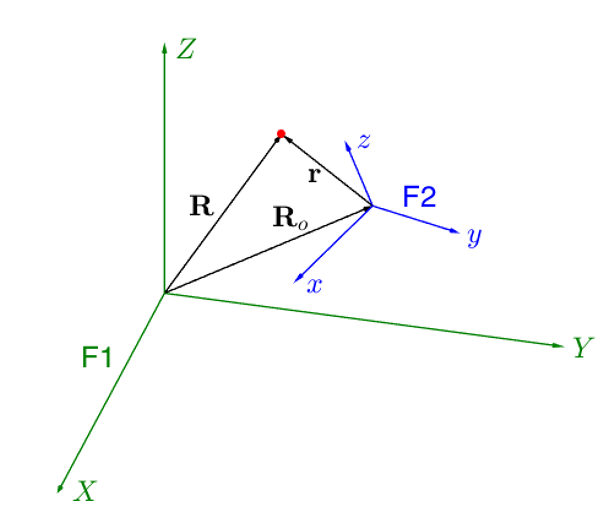
\includegraphics[scale=0.8]{AerospaceApplications/images/RFs.png}
\end{figure}

\noindent
In the above figure the following quantities are shown and a generic particle {\color{red}(in red)} is drawn: 
\begin{equation}
    \begin{aligned}
        &\mathbf{R} = X\mathbf{I} + Y \mathbf{J} + Z \mathbf{K}
        &\text{Position of the particle in F1}\\
        &\mathbf{r} = x \mathbf{i} + y \mathbf{j} + z \mathbf{k}
        &\text{Position of the particle in F2}\\
        &\mathbf{R_O}=X_O \mathbf{I} + Y_O \mathbf{J} + Z_O \mathbf{K}
        &\text{Position in F1 of the O of F2}
    \end{aligned}
\end{equation}
From the geometry follows that $\mathbf{R=R_O+r}$. One wonder at this point \textbf{what is the relation between $X$, $Y$, $Z$ and $x$, $y$, $z$}, using the given former properties we can write:
\begin{equation*}
    \begin{aligned}
        &X = \mathbf{R \cdot I} = \mathbf{(R_O+r) \cdot I} = 
        X_O + x\mathbf{I \cdot i} + y\mathbf{I \cdot j} + 
        z\mathbf{I \cdot k}\\ 
        &Y = \mathbf{R \cdot J} = \mathbf{(R_O+r) \cdot J} = Y_O + x\mathbf{J \cdot i} + y\mathbf{J \cdot j} + 
        z\mathbf{J \cdot k} 
         \\
        &Z = \mathbf{R \cdot K} = \mathbf{(R_O+r) \cdot K} =Z_O + x\mathbf{K \cdot i} + y\mathbf{K \cdot j} + 
        z\mathbf{K \cdot k} \\    
    \end{aligned}
\end{equation*}

Expressed in matrix form:

\begin{equation*}
    \begin{bmatrix}
        X\\Y\\Z
    \end{bmatrix} = 
    \begin{bmatrix}
        X_O\\Y_O\\Z_O
    \end{bmatrix}+
    \begin{bmatrix}
        \mathbf{I \cdot i}&\mathbf{I \cdot j}&\mathbf{I \cdot k}\\
        \mathbf{J \cdot i}&\mathbf{J \cdot j}&\mathbf{J \cdot k}\\
        \mathbf{K \cdot i}&\mathbf{K \cdot j}&\mathbf{K \cdot  k }
    \end{bmatrix}
    \begin{bmatrix}
        x\\y\\z
    \end{bmatrix}, \mathbf{T} \doteq \begin{bmatrix}
        \mathbf{I \cdot i}&\mathbf{I \cdot j}&\mathbf{I \cdot k}\\
        \mathbf{J \cdot i}&\mathbf{J \cdot j}&\mathbf{J \cdot k}\\
        \mathbf{K \cdot i}&\mathbf{K \cdot j}&\mathbf{K \cdot  k }
    \end{bmatrix}
\end{equation*}
The dot products $\mathbf{I \cdot i}$, $\mathbf{I \cdot j}$... represents the \textbf{direction cosine angles} which the axis of one reference frame forms with respect to the other. $\mathbf{T}$ is the \textit{direction cosine matrix}(\textbf{DCM}). 
In literature the DCM can be expressed as:
\begin{equation*}
  \mathbf{T}=\begin{bmatrix}
        T_{11}&T_{12}&T_{13}\\
        T_{21}&T_{22}&T_{23}\\
        T_{31}&T_{32}&T_{33}
    \end{bmatrix}=[T_{ij}]
\end{equation*}
and from the moment that translation and rotation can be studied indipendently, without loss of generality we can assume $\mathbf{R}_O=0$, then the $\mathbf{T}$ becomes a \textbf{transformation matrix} and in particular
\begin{equation*}
    \begin{bmatrix}
        \ X \ \\ \ Y \ \\\ Z \
    \end{bmatrix} = 
    \mathbf{T} 
    \begin{bmatrix}
       \ x \ \\ \ y \ \\ \ z \
    \end{bmatrix}
\end{equation*}
Furthermore, there are \textit{two different interpretation:}
\begin{itemize}
    \itemsep0em
    \item \textbf{Coordinate transformation} from F2 to F1 another term used to indicate this concept is \textit{alias}; 
    \item \textbf{Rotation} of vectors in a given fixed frame, so from F1 to F2, where F2 is the fixed one, another term to indicate this is \textit{alibi}.
\end{itemize}

\subsubsection*{\color{red} Some examples}
Let us consider some examples in 2D, the DCM assumes the form:
\begin{equation*}
    \mathbf{T} = \begin{bmatrix}
        \cos\theta&-\sin\theta\\
        \sin\theta&cos\theta
    \end{bmatrix}
\end{equation*}
From the moment that $z=0$, the third row and the third column of the complete matrix $\mathbf{T}$ disappear.\\

\noindent
{\color{blue} 
\textbf{(\#1) 2D-Coordinate transformation (alias) F2$\to$F1}
}\\
Let us assume that a reference frame F2 is rotated with respect to F1 of an angle $\theta=0.15\pi$, and a particle in F2 is given by
\begin{equation*}
    \mathbf{r} = 0.5\mathbf{i}+0.3\mathbf{j} =
    \begin{bmatrix}
        0.5\\0.3
    \end{bmatrix}
\end{equation*}
The particle coordinates in F1 are obtained through the following transformation
\begin{equation*}
    \begin{bmatrix}
        \ X \ \\ \ Y \
    \end{bmatrix} = \mathbf{Tr} 
\end{equation*}

\begin{figure}[h]
    \centering
    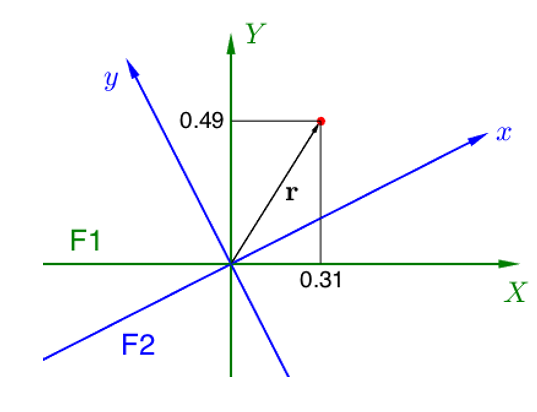
\includegraphics[scale=0.6]{AerospaceApplications/images/coord_transf.png}
    \caption{1st interpretation: Coordinate transformation}
\end{figure}

\noindent
{\color{blue} \textbf{(\#2) 2D-Rotation (alibi) F1$\to$F2}}\\
This time, let us consider a \textbf{vector} $\mathbf{r}$ that in the reference frame F2 is represented by
\begin{equation*}
    \mathbf{r} = \begin{bmatrix}
        \ 0.5 \ \\
        \ 0.3 \
    \end{bmatrix}
\end{equation*}
We can obtain a \textbf{rotated vector} $\mathbf{r}'$ in the same reference frame(fixed) applying the transformation $\mathbf{T}$: 
\begin{equation*}
    \mathbf{r}'=\mathbf{T}\cdot\mathbf{r}
\end{equation*}

\begin{figure}[h]
    \centering
    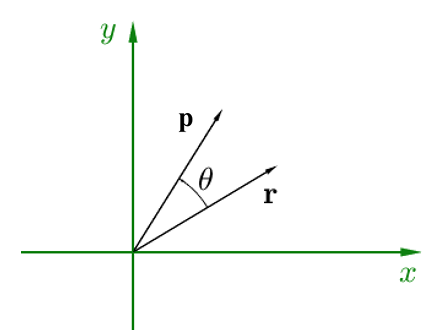
\includegraphics[scale=1]{AerospaceApplications/images/rotation_transf.png}
    \caption{2nd interpretation: rotation in a fixed frame}
\end{figure}

\noindent
{\color{blue} \textbf{(\#3) Rotation of a square in 2D}}
The concept of rotation can be generalized to a 2D-figure like a square for example. A square in 2D can be represented by a matrix $\mathbf{S}\in\mathbb{R}^{2,4}$, which contains by column the (2D)coordinates of the vertices.\\
If we want rotate a square of an angle $\theta$ we can apply the DCM (computed in the angle $\theta$) obtaining a \textbf{rotated square} $\mathbf{S'}$ as follows:
\begin{equation*}
    \mathbf{S'} = \mathbf{T} \cdot \mathbf{S}
\end{equation*}

\begin{figure}[h]
    \centering
    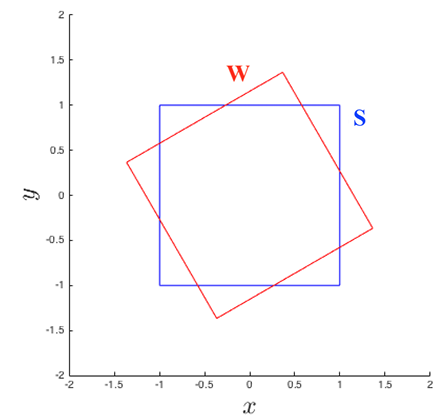
\includegraphics[scale=1]{AerospaceApplications/images/square_rot.png}
    \caption{Rotation of a square}
\end{figure}

\subsection{Euler angles}
In \textbf{three dimensions} we define the \textit{elementary rotation matrices}
\begin{equation*}
    \begin{aligned}
        &\mathbf{T}_1(\phi) = 
        \begin{bmatrix}
            1&0&0\\
            0&\cos\phi&-\sin\phi\\
            0&\sin\phi&cos\phi
        \end{bmatrix} & \text{Rotation about $X$ (or x) of $\phi$ }\\
        &\mathbf{T}_2(\theta) = 
        \begin{bmatrix}
            \cos\theta&0&\sin\theta\\
            0&1&0\\
            -\sin\theta&0&\cos\theta
        \end{bmatrix}  & \text{Rotation about $Y$ (or y) of $\theta$ } \\
        &\mathbf{T}_3(\psi) = \begin{bmatrix}
            \cos\psi&-\sin\psi&0\\
            sin\psi&cos\psi&0\\
            0&0&1
        \end{bmatrix}
        & \text{Rotation about $Z$ (or z) of $\psi$ }\\
    \end{aligned}
\end{equation*}
The interesting thing is that \textbf{any rotation in 3D} can be expressed as a product of $\mathbf{T}_1$, $\mathbf{T}_2$, $\mathbf{T}_3$, moreover the three angles $\phi, \theta, \psi$ are the so-called \textbf{Euler angles}.\\
There are 12 possible combinations of the three elementary matrices of rotations (with non sequentially repeated indexes) they can be divided in \textbf{two groups}: 
\begin{itemize}
    \itemsep0em
    \item[\ding{70}] \textbf{6 Tait-Bryan rotations} the most used are 123 and 321
    \item[\ding{70}] \textbf{6 proper Euler rotations} the most common is 313
\end{itemize}

As they are very used their expression is reported below:

{\color{red}\subsubsection{Tait-Bryan $\mathbf{T}_{123}$}}
\begin{equation*}
    {\large{
        \mathbf{T}_{123}=\begin{bmatrix}
            \cos\theta \cos \psi &
            -cos\theta \sin \psi &
            \sin\theta \\
            \cos\phi\sin\psi + \sin\phi\sin\theta\cos\psi&
            \cos\phi\cos\psi - \sin\phi\sin\theta\sin\psi&
            -\sin\phi\cos\theta\\
            \sin\phi\sin\psi-\cos\phi\sin\theta\cos\psi &
            \sin\phi\cos\psi+\cos\phi\sin\theta\sin\psi &
            \cos\phi\cos\theta
        \end{bmatrix}
    }}
\end{equation*}

{\color{red}\subsubsection{Tait-Bryan $\mathbf{T}_{321}$}}
\begin{equation*}
    {\large{
        \mathbf{T}_{321} = \begin{bmatrix}
            \cos\theta \cos\psi & -\cos\phi \sin\psi +\sin\phi\sin\theta\cos\psi & \sin\phi\sin\psi +\cos\phi \sin\theta \cos\psi\\
            \cos\theta \sin\psi & \cos\phi \cos\psi +\sin\phi\sin\theta\sin\psi & -\sin\phi\cos\psi +\cos\phi \sin\theta \sin\psi\\
            -\sin\theta & \sin\phi\cos\theta&\cos\phi\cos\theta
        \end{bmatrix}
    }}
\end{equation*}


{\color{red}\subsubsection{Proper Euler $\mathbf{T}_{313}$}}
\begin{equation*}
    {\large{
        \mathbf{T}_{313} = \begin{bmatrix}
            \cos\phi \cos\psi - \sin\phi \cos\theta \sin\psi & -\cos\phi \sin\psi -\sin\phi \cos\theta \cos\psi & \sin\phi \sin\theta\\
            \sin\phi \cos\psi + \cos\phi \cos\theta \sin\psi & -sin\phi \sin\psi + \cos\phi \cos\theta \cos\psi & -cos\phi \sin\theta\\
            \sin\theta \sin\psi & \sin\theta \cos\psi & \cos\theta 
    \end{bmatrix}
    }} 
\end{equation*}

\subsection{Rotation matrices general properties}
The following are \textbf{general properties} related to the rotation matrices. \textbf{Notation}: we indicate with $\mathbf{T}_{\diamond}$ any composition of the elementary rotation matrices (with non-sequentially repeated elements).\\
Matrices $\mathbf{T}_{\diamond}$ have the following properties:
\begin{itemize}
    \itemsep0em
    \item[\ding{70}] They are \textbf{linear transformations}, from the product of linear matrices;
    \item[\ding{70}] They are \textbf{orthogonal matrices}, that is matrices whose columns are composed of real entries and are \textbf{orthonormal}. The most important property is: 
    $$\mathbf{T}_{\diamond}^T=\mathbf{T}_{\diamond}^{-1}, \quad 
    \mathbf{T}_{\diamond}^{T}\mathbf{T}_{\diamond}=\mathbf{T}_{\diamond}\mathbf{T}_{\diamond}^T=\mathbf{I}$$
    \textbf{orthogonal transformations} preserve:
    \begin{itemize}
        \itemsep0em
        \item the \textbf{length} of the vectors;
        \item the \textbf{angles} between the vectors;
    \end{itemize}
    $$\text{length} + \text{angles} \Longrightarrow \textbf{shape preserved}$$
    \item[\ding{70}] Their \textbf{eigenvalues} are always $\{1, \pm e^{j\beta}\}$, their \textbf{determinant} always equal to 1;
\end{itemize} 

{\color{blue}\subsubsection{Singularities, Gimbal lock}}
For certain values of $\theta$ some matrices can present some \textbf{singularities}, for example the matrix $\mathbf{T}_{123}$. For example if $\theta=\frac{\pi}{2}$ only the sum $(\psi+\phi)$ can be determined and this results in a \textbf{loss of degree of freedom} $\Longrightarrow$ this phenomenon is also known as \textbf{gimbal lock} and affect all the \textit{gyroscopes} in which two out of three axes are aligned and this results in a loss of a degree of freedom, in \textit{normal situations} the three axis, instead, can rotate indipendently.
In order to overcome this problem, we use non minimal representation in which instead of only three variables, are used \textbf{four variables}.\\
More in general, \textbf{there is always a gimbal lock} when: 
\begin{itemize}
    \itemsep0em
    \item[\ding{70}] In the \textbf{Tait-Bryan rotations}, $\cos\theta=0$;
    \item[\ding{70}] In the \textbf{Proper Euler rotations}, when occurs that $\sin\theta=0$   
\end{itemize}
This singularities cause problems in the \textit{kinematic equation} like divergent behaviour, this is the reason why alternative method to manage these situations are required.

\begin{figure}[h]  
    \centering
    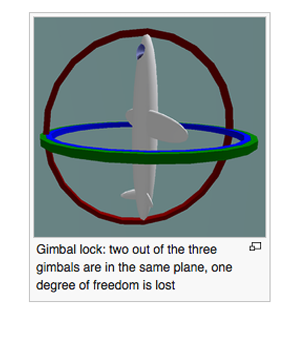
\includegraphics[scale=1.3]{AerospaceApplications/images/gimbal_lock.png}
    \caption{Gimbal lock example}
\end{figure}

\subsection{Euler's rotation theorem}
The following theorem is very important because it introduces an alternative way to describe rotations: \\

\hspace*{-5mm}
\begin{tikzpicture}
\node [mybox] (box){%
    \begin{minipage}{.96\textwidth}     %Larghezza del box
        \large{
            \textbf{\underline{Theorem (angle-axis representation)}}
            \begin{itemize}
                \itemsep0em
                \item[(i)] Any rotation of a rigid body where a point is fixed is \textbf{equivalent} to a rotation in which the rotation axis passes through the fixed point; 
                \item[(ii)] The rotation axis is the \textbf{eigenvector} $\mathbf{u}$ corresponding to the eigenvalues 1 of the rotation matrix. 
                \vspace{0.2cm}
            \end{itemize} 
        }
    \end{minipage}
};
\end{tikzpicture}%

\vspace{0.5cm}
\noindent
\textbf{\textit{Proof}}\\
The rotation matrix $\mathbf{T}_{\diamond}$ has a unitary eigenvalue, it holds (from the definition) that: $\mathbf{T}_{\diamond}\mathbf{u}=\mathbf{u}$, so the rotation does not change the direction $\mathbf{u}$, which is the rotation axis. $_\square$\\

From this theorem, follows that \textit{any rotation} can be described by using two quantities involving four variables: 
\begin{itemize}
    \itemsep0em
    \item[\ding{70}] An angle $\beta$ (1 variable)
    \item[\ding{70}] A rotation axis $\mathbf{u}$ (3 variables)
\end{itemize}
\huge{
\begin{equation*}
    \mathbf{T} \equiv \mathbf{T}(\beta, \mathbf{u})
\end{equation*}}





\subsection{Quaternions}